- TGS methods

- Elastodynamic methods
Du (2017)

Materials are modelled as anisotropic unbounded media (Fig. \ref{fig:seis-refl-tech}) through which elastic waves propagate according to the elastodynamic wave equation:
\begin{equation}
    C_{ijkl} \frac{\partial U_l(\vec{r},t)}{\partial x_j\partial x_k}= \rho(\vec{r},t)\frac{\partial U_l(\vec{r},t)}{\partial t^2}
    \label{eqn:ewe}
\end{equation}

where $C_{ijkl}$ are fourth-order stiffness tensor entries (Eqn. \ref{eqn:stiffness-full-notation}-\ref{eqn:stiffness-voigt-notation}) that are permutatively indexed by $i,j,k,l=1,2,3$ (Eqn. \ref{eqn:stiffness-full-notation}-\ref{eqn:stiffness-voigt-notation}), $\rho$ is density, $U$ is wave function.

The elastic tensor is calculated using a variable cell relaxation algorithm that consists of a loop over iterative SCF calculations while adjusting atomic positions and lattice constants. Elasticity theory relates the strain applied to the unit cell to the resulting calculated stress as an inverse problem, which could be solved using a non-linear solver with prior data as an initial guess vector. Deterministic thermoelastic relationships \cite{nyawere2014first} are also used to calculate elastic tensors from  changes in total energy and volume using \textit{ab initio} stress calculations.

\begin{figure}[h!]
    \centering
    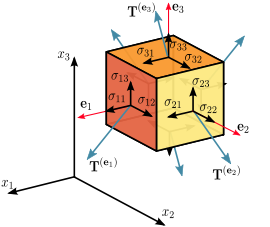
\includegraphics[width=0.6\textwidth]{Parts/Figures/Cij.png}
    \caption{Stress tensor visualization. (Source: S.A.F. Al Dajani. S.M. Thesis.) \cite{al2020non}}
    \label{fig19}
\end{figure}

The stress matrix calculated from density functional theory is used to calculate to the stress vector, which is the solution to the inverse problem comprised of the stiffness matrix and strain applied to the unit cell. This inverse problem is solved using linear algebra iteratively or using statistical thermoelastic physics that describe the system and depends on the symmetry of the system. In this case, nine distortions are applied to the unit across the principal axes of the orthorhombic crystal space group. These result in inputs to nine independent thermoelastic relationships that are used to calculate the elastic tensor. 

Both methods are used in a self-consistent fashion to converge to a solution that solves the elasticity inverse problem, $\underline{C}\vec{\epsilon} = \vec{\sigma}$, as follows: \cite{timoshenko1951theory, mit1620}

\begin{comment}
\begin{figure}[h!]
    \centering
    \includegraphics[width=0.8\textwidth]{elasticity.png}
    \caption{Stress-strain relationship and stiffness tensor. Source: Timoshenko, Theory of Elasticity \cite{timoshenko1951theory}}
    \label{fig:stiffness-tensor}
\end{figure}
\end{comment}




\begin{equation} \label{eqn:stiffness-full-notation}
\begin{bmatrix}
C_{1111} & C_{1122} & C_{1133} & C_{1123} & C_{1113} & C_{1112} \\
 & C_{2222} & C_{2233} & C_{2223} & C_{2213} & C_{2212} \\
 &  & C_{3333} & C_{3323} & C_{3313} & C_{3312} \\
 &  &  & C_{2323} & C_{2313} & C_{2312} \\
 & symm &  &  & C_{1313} & C_{1312} \\
 &  &  &  &  & C_{1212} 
\end{bmatrix} \begin{bmatrix}
\epsilon_{11} \\
\epsilon_{22} \\
\epsilon_{33} \\
2\epsilon_{23} \\
2\epsilon_{13} \\
2\epsilon_{12} 
\end{bmatrix}  =  \begin{bmatrix}
\sigma_{11} \\
\sigma_{22} \\
\sigma_{33} \\
\sigma_{23} \\
\sigma_{13} \\
\sigma_{12} 
\end{bmatrix}  
\end{equation} 
or in Voigt notation:
\begin{equation} \label{eqn:stiffness-voigt-notation}
 \begin{bmatrix}
C_{11} & C_{12} & C_{13} & C_{14} & C_{15} & C_{16} \\
 & C_{22} & C_{23} & C_{24} & C_{25} & C_{26} \\
 &  & C_{33} & C_{34} & C_{35} & C_{36} \\
 &  &  & C_{44} & C_{45} & C_{46} \\
 & symm &  &  & C_{55} & C_{56} \\
 &  &  &  &  & C_{66} 
\end{bmatrix}  \begin{bmatrix}
\epsilon_{1} \\
\epsilon_{2} \\
\epsilon_{3} \\
\epsilon_{4} \\
\epsilon_{5} \\
\epsilon_{6} 
\end{bmatrix}  =  \begin{bmatrix}
\sigma_{1} \\
\sigma_{2} \\
\sigma_{3} \\
\sigma_{4} \\
\sigma_{5} \\
\sigma_{6} 
\end{bmatrix}  
\end{equation}


- DFT methods

Material properties are calculated from a self-consistent, non-linear field calculation, (Fig. \ref{fig:scf-loop}) which is a variational method that optimizes over charge density that adjusts atomic positions until a threshold in energy minimization is achieved in a simplified ion-core model of atoms and electrons in a given material to solve the many-body wave equation. \cite{Schwingenschloegl2004} Electron dispersion is calculated using a non-consistent field calculation to interpolate the energy calculations in momentum space. The phonon dispersion is calculated from the dynamical matrix obtained from \textit{ab initio} calculations. \cite{hung2022quantum, giustino2014materials}

Self-consistent, non-linear field calculation algorithms calculate external potentials with a Poisson equation solver, (Fig. \ref{fig:scf-loop}) which depends on simulation geometry, atomic positions of ions, pseudopotentials used for the atoms involved, and other inputs. This external potential (Fig. \ref{fig:poisson-hartree-potential}) is then used as a guess for the electron density with a Schr\"{o}dinger equation solver, (Fig. \ref{fig:schrodinger-electron-density}) which is then used as inputs to a self-consistent field loop that calculates the charge density iteratively to minimize the total energy. The accuracy of this algorithm depends on the cut-off applied to the energy minimization, the charge density, the size of the momentum grid, and other convergence thresholds on the outputs. \cite{hung2022quantum, Schwingenschloegl2004, giustino2014materials}

In order to model the BCC Fe--Cr $\delta$--ferrite solid solution, the sequential quasirandom structure (SQS) methodology was employed \cite{VandeWalleLiu2013}. 
The \texttt{mcsqs} software package within the Alloy Theoretic Automated Toolkit (ATAT) was used in order to generate SQS supercells.
The Vienna \textit{ab initio} Simulation Package (VASP) was used to perform the density functional theory (DFT) total energy calculations, which were used to derive the elastic properties as well as the enthalpy of mixing. 
Spin--polarized DFT calculations were performed on 40--atom SQS supercells employing $\Gamma$--point sampling of reciprocal space along with a 500 eV planewave cutoff energy. 
The Projector--Augmented Wave (PAW) method was employed for the ionic pseudopotential, and the Perdew--Burke--Ernzenhoffer parameterization of the Generalized Gradient Approximation (GGA) of the exchange--correlation functional. 

- Analysis of DFT results

With the elastic tensor obtained from quantum mechanical calculations, elastic moduli could be calculated. Korzhavyi et al. (PRB, 2009) and Razumovskiy et al. (PRB, 2011) highlight the significance of elastic moduli in characterizing material behavior and report the elastic constants of iron-chrome with increasing chromium content using density functional theory. By considering embrittlement criteria, the propensity of materials to undergo embrittlement could be evaluated to assess their mechanical stability.

\begin{eqnarray}
    C' = \frac{C_{11}-C{12}}{2} \\
    B = \frac{C_{11} + 2C+{12}}{3} \\
    \Rightarrow C_{11}= \frac{3B+4C'}{3} \\
    \Rightarrow C_{12} = C_{11} - 2 C' \\ \\
    G_V = \frac{C_{11}-C_{12} + 3C_{44}}{5} \\
    G_R = \frac{5(C_{11}-C_{12})C_{44}}{4C_{44}+3(C_{11}-C_{12})} \\ \\
    G = \frac{G_V + G_R}{2} \\
    E = \frac{9BG}{3B+G} \\
    \nu = \frac{3B-E}{6B}
\end{eqnarray}
ADD equations for Rayleigh wave and acoustic wave frequencies
Figure out to use K or G for shear modulus


- Embrittlement prediction

- Stiffening prediction

- Inferring plasticity from elasticity with melting point

- Probability dist methods

\begin{comment}
Spin polarized first--principles density functional theory (DFT) calculations were conducted using the Vienna 
\emph{Ab initio} Simulation Package (VASP) \cite{Kresse1996,Hafner2008}. 
%
A plane--wave cutoff energy of 500 eV was used throughout the calculations, along with a $\Gamma$--centered 7x7x7 k--point grid to sample the Brillouin zone.
%
The total energy of the pristine supercell was found to converge to within 5 meV under these conditions. 
%
The projector augmented--wave (PAW) pseudopotentials were used to describe the ion--electron interactions \cite{Blochl-1994-PAW,Kresse-Joubert-1999-PAW}. 
%
The Perdew--Burke--Ernzerhof parameterization of the generalized gradient approximation (GGA) exchange--correlation functional, revised for use in solids (PBEsol) was used \cite{PBE-PRL-1996,PBEsol}.
%
Additionally, relaxation of the supercell size, shape, and ionic positions was performed for both the pristine and vacancy--containing structures to account for the effect of local lattice distortion.



In order to physically represent the random solid solution HEAs, the sequential quasirandom structure (SQS) method was employed \cite{ZungerBernard1990}. 
% 
The SQS method has been shown to accurately predict the properties of disordered solids with supercells as small as 16 atoms \cite{Wolverton2001,Jiang2009,Saal2013,liu2016first,WANG201888}.
% 
Distinct 30 atom SQS supercells for both alloys were produced using the \texttt{mcsqs} code within the Alloy Theoretic Automated Toolkit \cite{VandeWalleLiu2013,VandeWalle2009}. 
% 
The SQS method differs from other popular methods for representing random solid solutions such as the coherent potential approximation (CPA) and the virtual crystal approximation (VCA) in that it is not an effective medium approach, and therefore the SQS method can provide detailed insights into the effect of local atomic structure within random solid solutions. 
%






\end{comment}